\section{METHODS}



\begin{figure}[schematic_finger_overhead]
  \label{fig:schematic_finger_overhead}
  \centering
  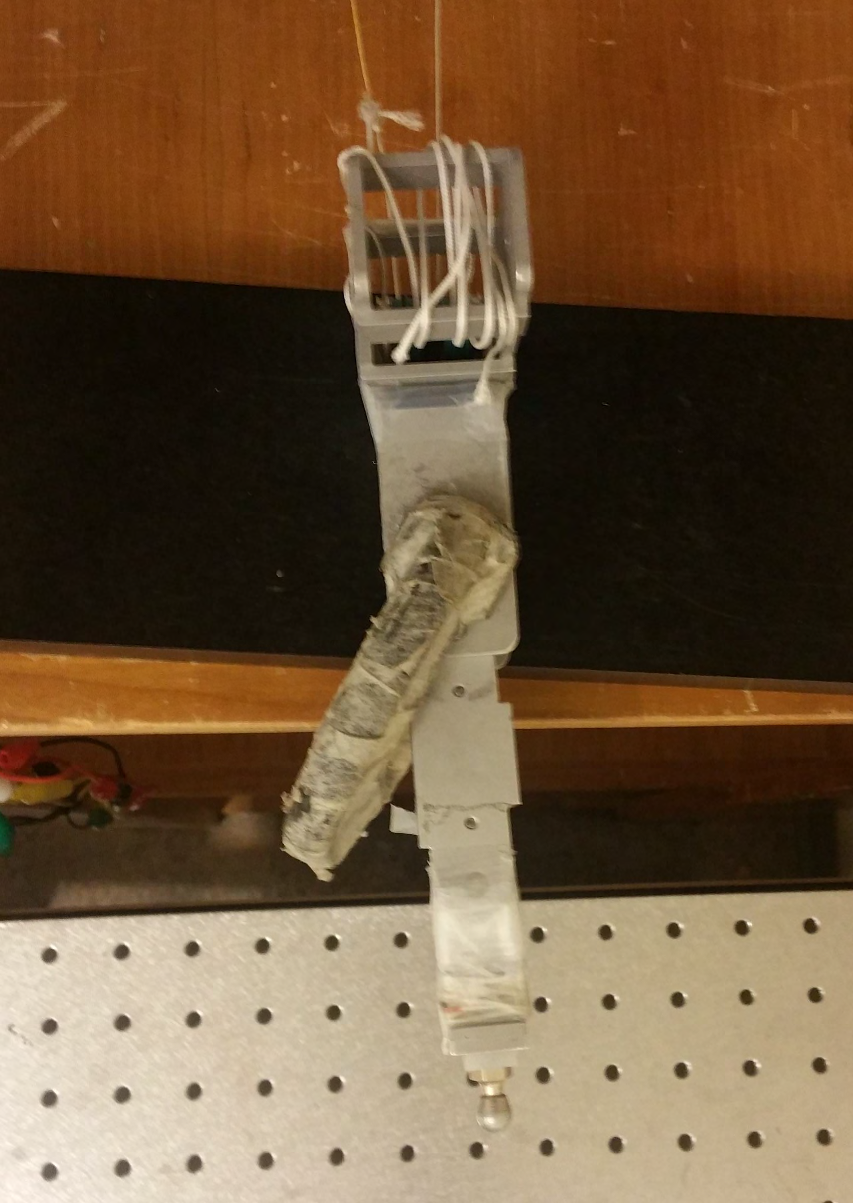
\includegraphics[width=0.5\textwidth]{figures/overhead_robotic_finger.pdf}
  \caption{Tendon driven robotic finger with one joint, 1DOF, 2 muscles}
\end{figure}

\begin{figure}[hardware_schematic]
  \label{fig:hardware_schematic}
  \centering
  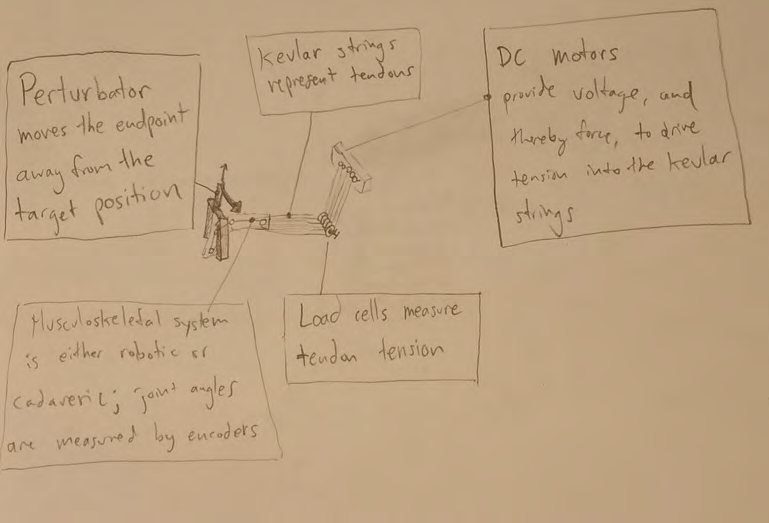
\includegraphics[width=1.0\textwidth]{figures/hardware_schematic.pdf}
  \caption{Caption one two three}
\end{figure}

\begin{figure}[fpga_schematic]
  \label{fig:fpga_schematic}
  \centering
  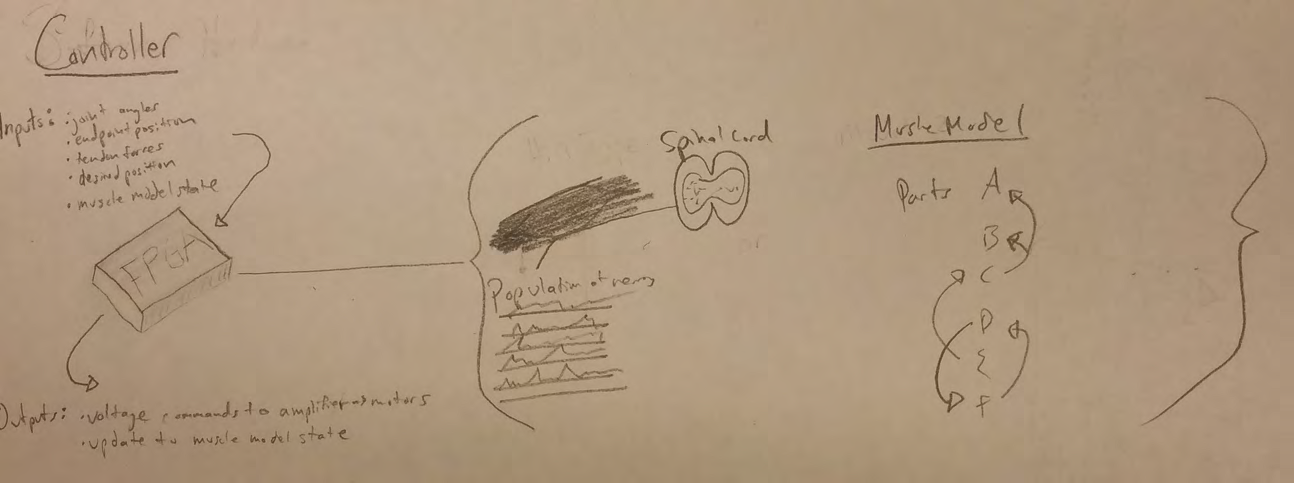
\includegraphics[width=1.0\textwidth]{figures/fpga_schematic.pdf}
  \caption{Caption one two three}
\end{figure}


\begin{figure}[loadcells_pulley]
  \label{fig:loadcells_pulley}
  \centering
  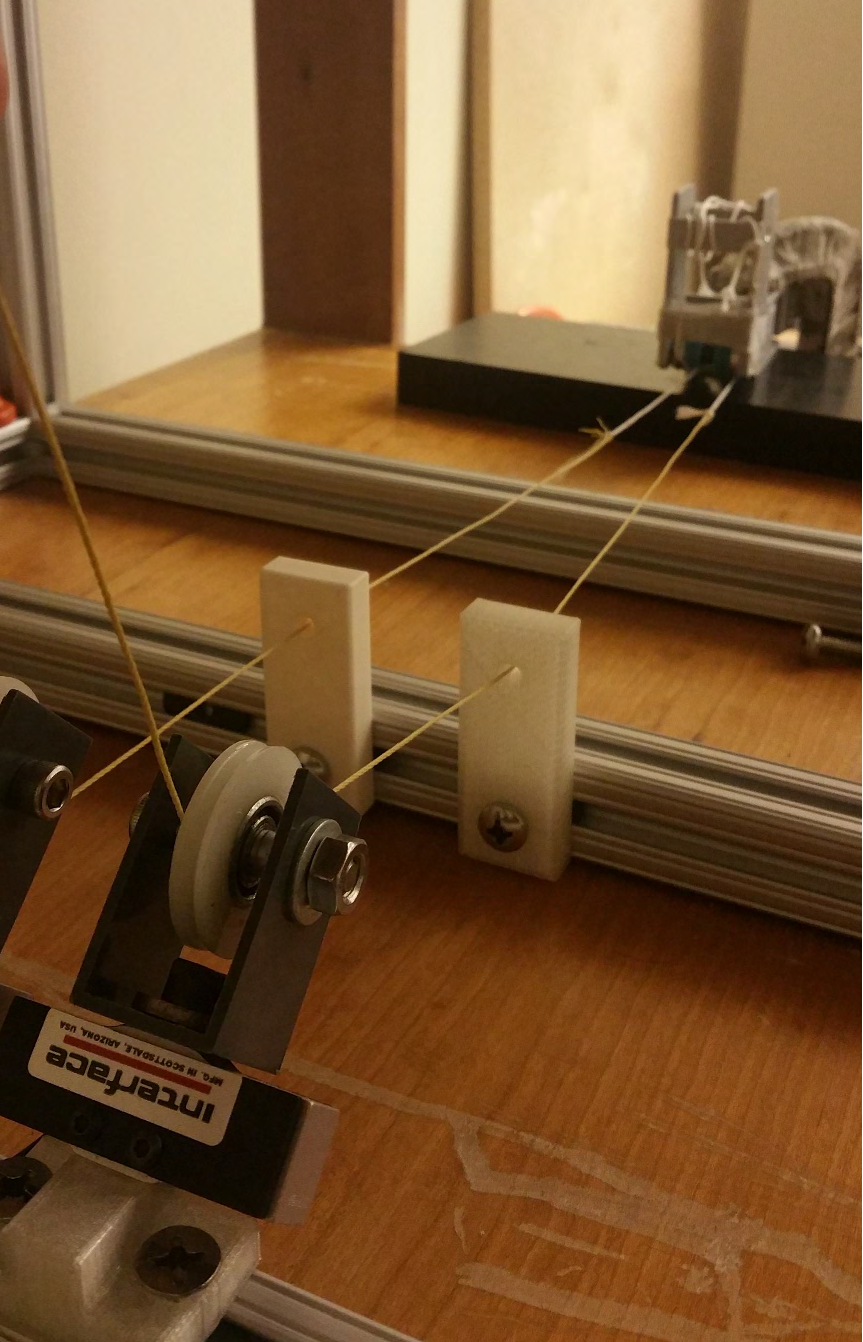
\includegraphics[width=0.5\textwidth]{figures/loadcells_pulley.pdf}
  \caption{Caption one two three}
\end{figure}
\begin{figure}[motor_closeup]
  \label{fig:motor_closeup}
  \centering
  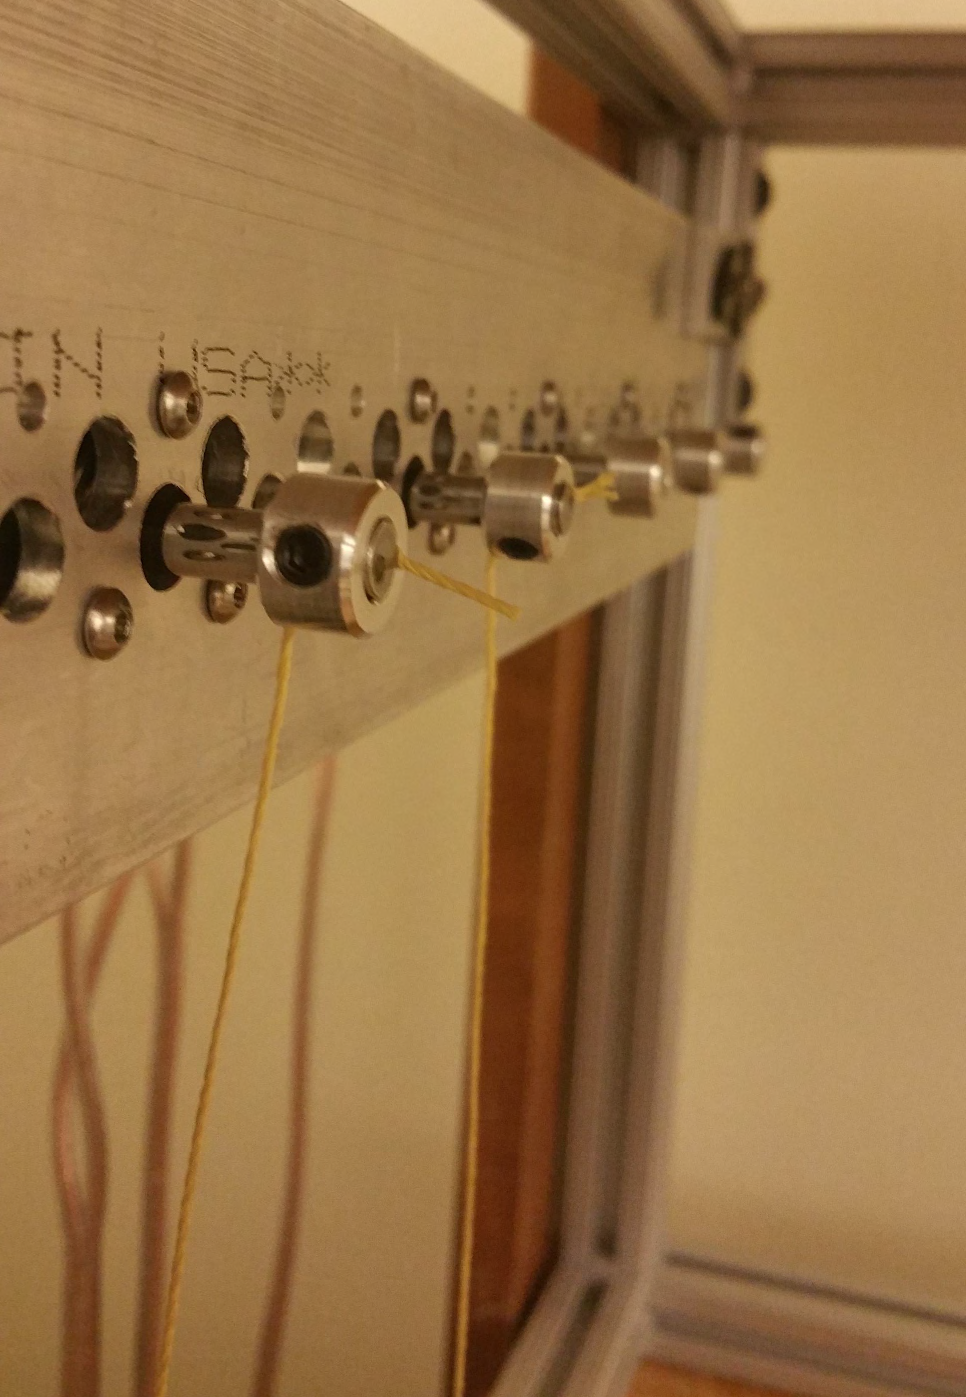
\includegraphics[width=0.5\textwidth]{figures/motor_closeup.pdf}
  \caption{Caption one two three}
\end{figure}
